\section{Sample Results}\label{sec.flowsheet.results.table}

Flowsheet evaluations that have been run in a FOQUS session can be viewed by clicking the table button in the flowsheet toolbar (\#13 in Figure \ref{fig.flowsheet.editor}). The results are displayed in a table, and the contents can be copied and pasted into a spreadsheet or exported to a CSV file. Figure \ref{fig.results.table} show the Flowsheet Results Table window.


\begin{figure}[H]
	\begin{center}
		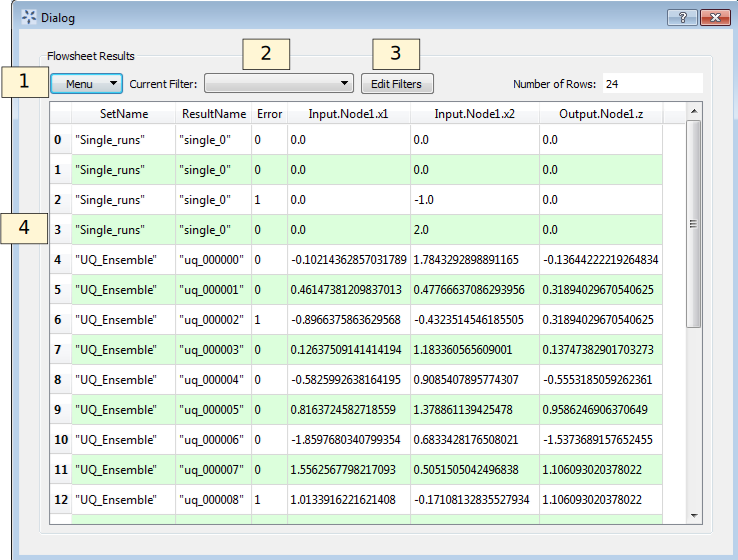
\includegraphics[scale=0.55]{Chapt_flowsheet/figs/resultsTable}
		\caption{Flowsheet Results Table Window}
		\label{fig.results.table}
	\end{center}
\end{figure}
\begin{samepage}
\begin{enumerate}
	\item \bu{Menu} contains a menu with four sub menus.
	\begin{enumerate}
		\item \bu{Import} data from files or the clipboard.
		\item \bu{Export} data to files or the clipboard.
		\item \bu{Edit} or delete data.
		\item \bu{View} options for the table.
	\end{enumerate}
	\item The \textbf{\underline{Current Filter}} drop-down list enables the user to select a data filter, which can be used to filter and sort data.
	\item \bu{Edit Filters} enables the user to create or edit data filters.
\end{enumerate}
\end{samepage}

\subsection{Error Codes}
Error codes are listed in the \textbf{\underline{Flowsheet Results}} table for the whole flowsheet and for individual nodes. Table \ref{table.fs.error} shows the flowsheet error codes and Table \ref{table.node.error} shows the node error codes. The most common flowsheet error is 1, a node calculation failed. The most common node error is 7, Turbine simulation error. These errors are typically caused by a simulation that fails to converge or has some other calculation error (e.g., ACM does not converge or an Excel spreadsheet simulation with a division by 0 error). 

\begin{table}[H]
	\begin{center}
		\caption{Flowsheet Error Codes}\label{table.fs.error}
		\begin{tabularx}{4.5in}{r l}
			\hline
			Code & Meaning \\
			\hline
			-1 & Did not run or finish  \\
			 0 & Success \\
			 1 & A node calculation failed \\
			 3 & Failed to create a worker node \\
			 5 & Unknown tear solver \\
			11 & Wegstein failed to converge \\
			12 & Direct failed to converge \\
			16 & Presolve node error \\
			17 & Postsolve node error \\
			19 & Unhandled exception during evaluation (see log)\\
			20 & Flowsheet thread terminated \\
			21 & Missing session name \\
			40 & Error connecting to Turbine \\
			50 & Error loading session or inputs \\
			100 & Single node calculation success \\
			201 & Cycle in determining calculation order (invalid tear set) \\
			\hline
		\end{tabularx}
	\end{center}
\end{table}

\begin{table}[H]
	\begin{center}
		\caption{Node Error Codes}\label{table.node.error}
		\begin{tabularx}{4.5in}{r l}
			\hline
			Code & Meaning \\
			\hline
			-1 & Did not run or finish  \\
			0 & Success \\
			1 & Simulation error (see log) \\
			3 & Exceeded maximum wait time \\
			4 & Failed to create Turbine session ID \\
			5 & Failed to add Turbine job \\
			6 & Exceeded maximum run time\\
			7 & Turbine simulation error \\
			8 & Failed to start Turbine job \\
		   10 & Failed to get Turbine jobs status \\
		   11 & Flowsheet thread terminated \\
		   20 & Error in node script\\
		   23 & Could not convert Numpy value to list \\
		   27 & Cannot read variable result (see log)\\
			\hline
		\end{tabularx}
	\end{center}
\end{table}